%%%%%%%%%%%%%%%%%%%%%%%%%%%%%%%%%%%%%%%%%%%%%%%%%%%%%%%%%%%%%%%%%%%%%%%%%%%%%%%%%%
\begin{frame}[fragile]\frametitle{}
\begin{center}
{\Large LLM in Production}

{\tiny (Ref: MLOps.community channel on Youtube)}

\end{center}
\end{frame}

%%%%%%%%%%%%%%%%%%%%%%%%%%%%%%%%%%%%%%%%%%%%%%%%%%%%%%%%%%%
\begin{frame}[fragile]\frametitle{Compare before use}

\begin{center}
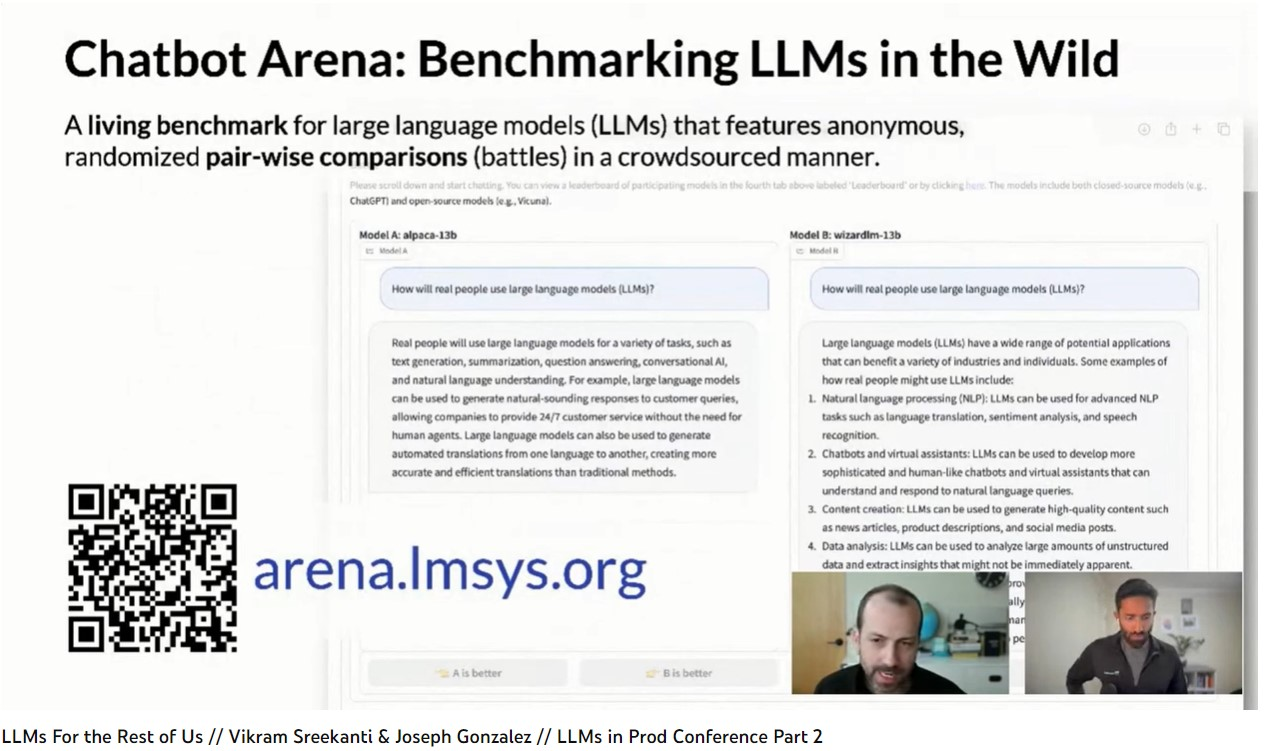
\includegraphics[width=\linewidth,keepaspectratio]{llm57}
\end{center}
\end{frame}

%%%%%%%%%%%%%%%%%%%%%%%%%%%%%%%%%%%%%%%%%%%%%%%%%%%%%%%%%%%
\begin{frame}[fragile]\frametitle{Missing Link}
\begin{columns}
    \begin{column}[T]{0.5\linewidth}
		\begin{itemize}
		\item Good models are hosted ones, so you tend to build own (foundation) model, do you really need it? Use largest that you can afford/use.
		\item Use your own data via Vector Databases
		\item Exhausting prompt engineering, chaining, orchestration frameworks.
		\item Be specific and not expect that models will do everything.
		\item Have good data quality and governance and also good Validation, tracing and logging.
		\end{itemize}	
    \end{column}
    \begin{column}[T]{0.5\linewidth}
		\begin{center}
			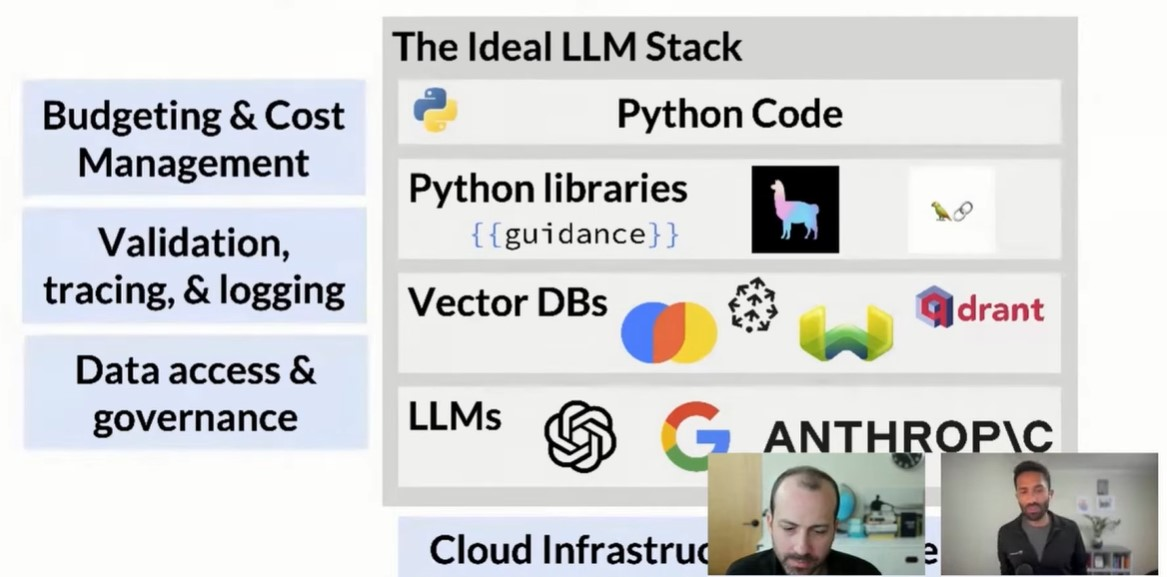
\includegraphics[width=\linewidth,keepaspectratio]{llm58}
		\end{center}
	\end{column}
  \end{columns}
\end{frame}


%%%%%%%%%%%%%%%%%%%%%%%%%%%%%%%%%%%%%%%%%%%%%%%%%%%%%%%%%%%
\begin{frame}[fragile]\frametitle{Customizing Solutions}

\begin{itemize}
\item Fine tuning: few shots, whole model
\item Hand crafted prompts
\item Optimization
	\begin{itemize}
	\item Programmatic prompt generation (human readable)
	\item AutoPrompt (Gradient based searches), not human readable
	\item Continuous: P-tuning, Prefix-tuning
	\end{itemize}
\item RLHF (Reinforcement Learning with Human Feedback)
\end{itemize}	

Which one is most appropriate? What about platforms which provide customization?
\end{frame}


%%%%%%%%%%%%%%%%%%%%%%%%%%%%%%%%%%%%%%%%%%%%%%%%%%%%%%%%%%%
\begin{frame}[fragile]\frametitle{Evaluation}

\begin{itemize}
\item `Hero` use cases ( say smoke test, must work)
\item White box testing
\item Edge cases, missing conflicting data
\item User feedback, bugs
\item Out of scope functionality, graceful denial.
\end{itemize}

{\tiny (Ref: Combining LLMs with Knowledge Bases to Prevent Hallucinations - Scott Mackie - LLMs in Prod Con 2 )}

\end{frame}

%%%%%%%%%%%%%%%%%%%%%%%%%%%%%%%%%%%%%%%%%%%%%%%%%%%%%%%%%%%
\begin{frame}[fragile]\frametitle{Shared Responsibility Model}

\begin{center}
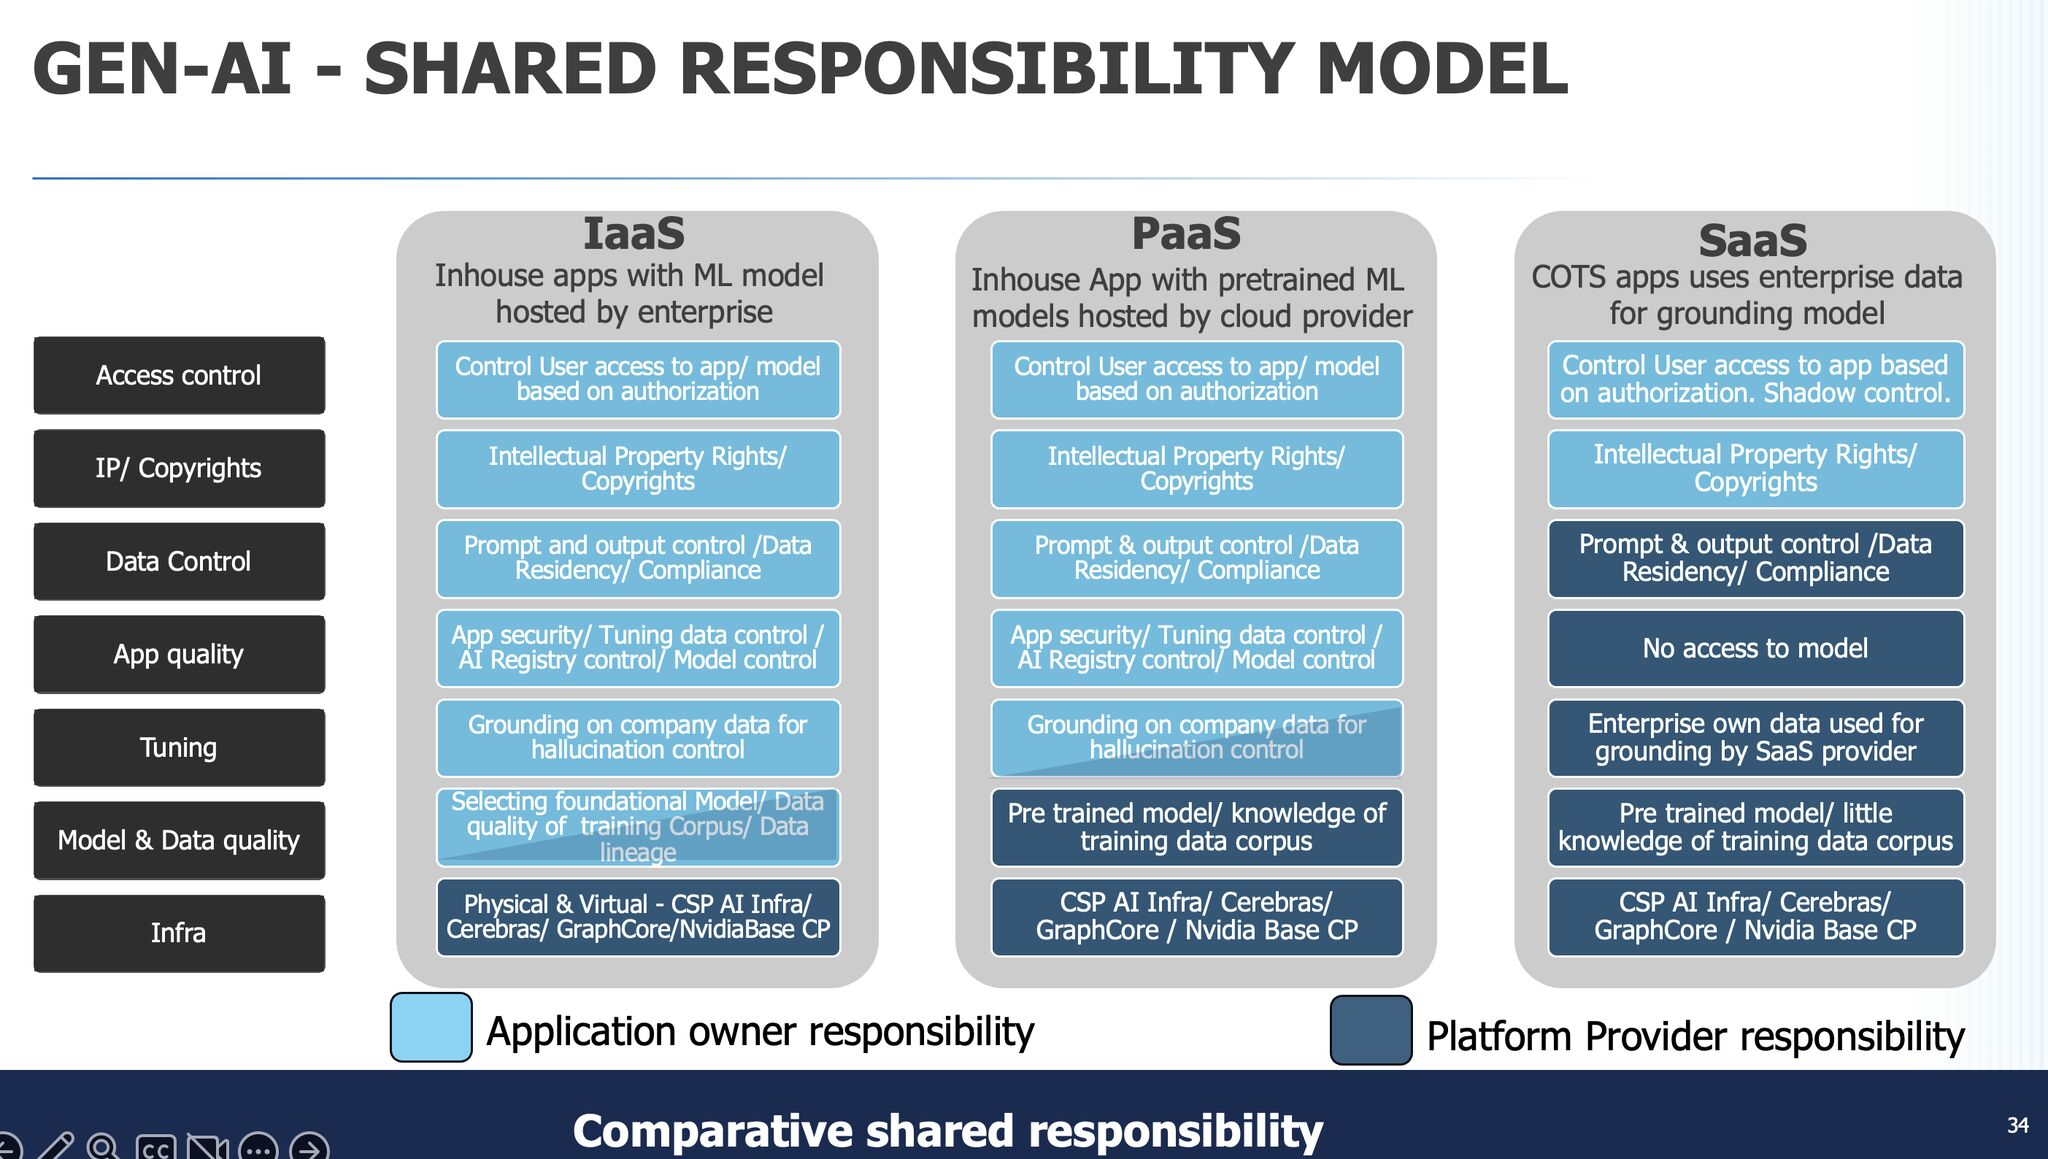
\includegraphics[width=\linewidth,keepaspectratio]{llm63}
\end{center}		


{\tiny (Ref: Linkedin Post on 11 Aug 2023 by - Vishwas Manral )}

\end{frame}


%%%%%%%%%%%%%%%%%%%%%%%%%%%%%%%%%%%%%%%%%%%%%%%%%%%%%%%%%%%
\begin{frame}[fragile]\frametitle{Commercial Example: Intuit GenOS}

\begin{itemize}
    \item GenStudio: Dev environment for rapid experimentation with generative AI experiences.
    \item GenRuntime: Intelligent layer choosing appropriate large language model in real time, based on user needs.
    \item GenUX: Library of UI components and user flows for clear and delightful interactions.
    \item Financial LLMs: Custom trained for tax, accounting, marketing, etc., providing insights and actions.
\end{itemize}

\end{frame}

